\noindent We begin by outlining the techniques used to effectively optimize 
unstructured mesh applications on GPUs -- some of which are well established 
and commonly used. We briefly show a na\"{i}ve solution, then continue 
with describing various improvements found in the literature, and then present 
our contributions.

\subsection{Traditional parallelization approaches}

\noindent On a GPU, groups of threads (warps) run at the same time, in 
lockstep. As such it is not efficient to execute computations of different 
length on different threads. Consequently, the usual practice is for each thread 
to take responsibility for the computation on one element of the set. This can 
be viewed as running one iteration per thread in the loop over a given set, also 
known as the iteration set or from-set. This allows the number of computations 
to be fixed, where the amount of data involved is fixed in the dimension of the 
mapping and the data arrays.

As mentioned before, care must be taken when writing parallel code to avoid 
data races when different threads modify the same data. There are three 
approaches discussed in the literature. The first is to color each thread 
according to the indirect data it writes, so that no two threads with the same 
color write the same data, and enforce ordering between colors using 
synchronization~\cite{Zegard2013}. On the GPU, one would do multiple kernel 
launches corresponding to the colors, so there is no concurrent writes between 
threads in the same kernel. We call this the \emph{global coloring} approach 
(Figure \ref{fig:unstructured_global}). The disadvantage here is that there is 
virtually no data reuse: when multiple elements write the same data, they are scheduled 
for execution in different launches. Since these operations also tend to read 
data through the same mappings, there is no data reuse in the reads either. 
Compounding the issue is low cache line utilization where elements of the same 
color are not neighbors in the mesh, and therefore unlikely to be stored in 
consecutive memory locations.

\begin{figure}[Htpb]
  \centering
  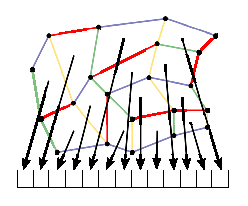
\includegraphics{fig/svg/unstructured_global.eps}
  \caption{Schematic figure of the global colouring approach. In each kernel
  launch, the kernels work on edges of the same colour. The arrows
  represent the individual pieces of data loaded indirectly when executing the color red.}
  \label{fig:unstructured_global}
\end{figure}

The second approach is to serialize the indirect updates by means of locks or
atomic additions \cite{Kraus:2014:ACC:2691158.2691164}. This is considerably 
expensive on the GPU, since the whole warp has to wait at the synchronization 
step leading to warp divergence.

The third solution is the use of a large temporary array that stores the
results for each thread separately, avoiding race conditions by formulation 
\cite{LULESH:spec,miniaero}. However, after the computation finishes, a 
further kernel is required to gather the results corresponding to one data 
point. This suffers from the problem of not knowing how many values one thread 
has to gather, and as a result warps could diverge significantly, and 
memory access patterns are less than ideal. They can be good either for the 
write or the read, but not for both. Also, the size of the temporary array is the 
number of elements multiplied by the dimension of the mapping. As a result, it 
can be large, for example, in LULESH, it is \(8 \times 3 \times numElem \) 
in our measurements (where $numElem$ is the size of the from-set in LULESH), 
compared to the array defined on nodes where these values will ultimately end 
up, which is roughly the same as the number of elements themselves.

\subsubsection{Array-of-Structures (AoS) vs Structure-of-Arrays (SoA)} 
\label{aos-to-soa}

Due to the lockstep execution, consecutive threads in a warp read  memory at
the same time. Therefore, the layout of the data in the memory is an important
factor for performance. There are two commonly used
layouts~\cite{sharma2015data}: (1) Array-of-Structures (AoS) layout, where the
data associated with one element is in consecutive places in the array (and thus
in memory) and (2) Structure-of-Arrays (SoA) where the components of elements
are stored consecutively e.g. the first data component of the elements are in
the beginning of the array followed by the second, etc.

Although in most cases the SoA gives better performance on GPUs and better
vectorization on CPUs, the AoS layout is still commonly used on CPU
architectures with large caches. In the case of the AoS layout, consecutive
threads read data from strided addresses in memory and thus more cache lines 
are required to satisfy one transaction. This would be compensated by 
subsequently reading the other components, but may have a negative effect on 
 GPUs due to their small caches. Conversely, with the SoA layout, the 
threads read data next to each other, which means that the data needed by 
consecutive threads are most probably in the same cache line resulting in 
coalesced memory transactions. However, when indirections are involved, these
access patterns become more complicated --- even with the SoA pattern,
consecutive threads may not be reading consecutive values in memory, and
therefore cache line utilization degrades. The choice of data layout in
unstructured mesh computations is therefore highly non-trivial, as we show
later.

\subsection{Shared memory approach}\label{shared-memory-approach}

Considering the three data race avoiding approaches, we see that they all only 
make use of the GPU global memory. As such one technique to further improve 
performance is by reducing memory accesses to the GPU global memory. To this 
end, the OP2 library~\cite{op2} targets the use of the shared memory on the 
GPUs. Shared memory is only shared within thread blocks, but has much lower 
access latency and higher bandwidth than the global memory. The idea is to 
collect the data required to perform the computations and load it into shared 
memory. Then, during computation, the indirect accesses are to the shared
memory, and the result can also be stored there. After computations by all 
threads in the block have completed, the contents of the shared memory can be 
written back to global memory. One immediate advantage of this approach is that 
the fetching and writing back of data from/to the global memory can be done by 
the threads independently of the actual threads that will be carrying out the 
computations on them. Particularly, reading/writing can be done in the order 
in which the data is laid out in memory, ensuring maximum utilization of 
cache lines. With the AoS layout, data can be read in contiguous chunks as 
large as the number of components in the structure.

The use of shared memory of course leads to one additional complication. 
Writing back the updated patches of shared-memory to GPU global memory may lead 
to data races. This leads to the use of a \emph{two-layered coloring} or 
\emph{hierarchical coloring}~\cite{op2} scheme. The two levels of coloring are illustrated in Figure \ref{fig:multilevel}, and the associated data accesses are shown in Figure \ref{fig:unstructured_hier}. The 
first level of coloring is to avoid data races when thread blocks write the result back to 
global memory and the second level is to avoid threads writing their results into 
shared memory at the same time. 

\begin{figure}[Htpb]
  \centering
  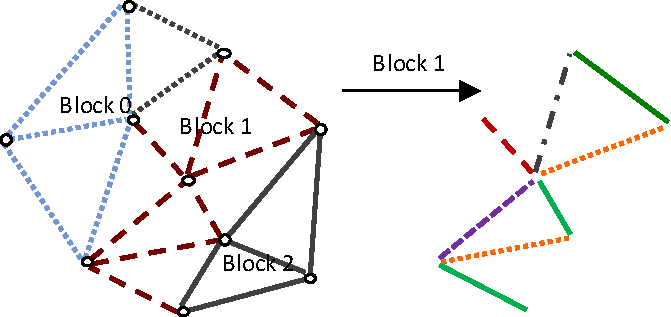
\includegraphics[width=0.5\textwidth]{fig/multilevel.pdf}
  \caption{Schematic figure of the two levels of coloring.}
  \label{fig:multilevel}
\end{figure}

\begin{figure}[Htpb]
  \centering
  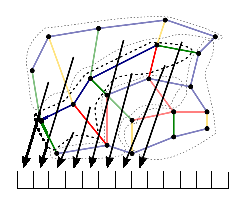
\includegraphics{fig/svg/unstructured_hier.eps}
  \caption{Schematic figure of the hierarchical coloring approach. The thread
  blocks are circled with dashed lines. The arrows represent the individual data
  points loaded.}
  \label{fig:unstructured_hier}
\end{figure}

Algorithm~\ref{code:shared} details the steps carried out by a CUDA kernel for
executing within this two-level coloring scheme. All indirect data accessed by
the block (which is identified during a preprocessing phase) is fetched from
global to shared memory to shared memory. As noted in Section~\ref{aos-to-soa},
data is usually composed of data points with multiple components (for example,
x-y-z coordinates), so this operation consists of two nested loops: (1) an
iteration over the data points, and within that, (2) an iteration over the data
corresponding to the data point. For the SoA layout, only the outer loop needs
to be parallelized, as this will cause parallel read operations to access memory
addresses next to each other. For the same reason, if the AoS layout is used,
both parallel loops need to be parallelized (i.e.  collapsed into one). The data
layout in shared memory is best be set to SoA: our measurements showed a
consistent degradation in performance when switching to AoS layout, due to the
spatial locality described in Section \ref{aos-to-soa}: it leads to fewer bank
conflicts.

After the data is loaded into shared memory, each thread executes the main body 
of the kernel, and outputs are placed into registers.  Next, the threads update 
the result in shared memory with their increments. Finally the updated data is 
written back to global memory.

\begin{algorithm}
  \begin{algorithmic}
    \State \lstinline!tid = blockIdx.x * blockDim.x + threadIdx.x!
    \State \lstinline!bid = blockIdx.x!
    \ForAll {\lstinline!data_point! $\in$ \lstinline!indirect_data!}
      \ForAll {\lstinline!d! $\in$ \lstinline!data_point!}
        \State \lstinline!shared[shared_ind(d)] = global_indirect[d]!
      \EndFor
    \EndFor
    \State \lstinline!__syncthreads()!
    \State \lstinline!result = computation(shared[mapping[tid]], global_direct[tid])!
    \State \lstinline!__syncthreads()!
    \State fill shared memory with zeros
    \State \lstinline!__syncthreads()!
    \For {\lstinline!c = 1! $\ldots$ \lstinline!num_thread_colours!}
      \If{\lstinline!c == thread_colours[tid]!}
        \State increment shared with result
      \EndIf
      \State \lstinline!__syncthreads()!
    \EndFor
    \ForAll {\lstinline!data_point! $\in$ \lstinline!indirect_data!}
      \ForAll {\lstinline!d! $\in$ \lstinline!data_point!}
        \State increment \lstinline!global_indirect_out! with shared
      \EndFor
    \EndFor
  \end{algorithmic}
  \caption{Algorithm to use the shared memory to preload indirect data accessed
  within a thread block. \lstinline!global_indirect! holds the data indirectly
  read, \lstinline!global_indirect_out! holds the result of the iteration.}
  \label{code:shared}
\end{algorithm}

One other benefit from using shared memory with hierarchical coloring is the 
improved data reuse within the block. Each piece of data has to be loaded 
from global memory only once, but can be used by multiple threads (e.g. data on 
a shared edge between two triangles). However, the greater the reuse, the more 
thread colors we have: the number of colors is no less than the number of 
threads writing the same data. Since the number of synchronizations also grows 
with the number of thread colors (more precisely, it is the number of colors 
plus two, one before and one after the computation if the input and the 
increment are stored separately in shared memory), there is a trade-off between 
the number of synchronizations and data reuse. Our measurements showed that if 
the kernel is memory-bound, the greater data reuse leads to increased 
performance, but the trade-off is non-trivial, as we will demonstrate in 
Section~\ref{performance}.

\subsection{Increasing data reuse}\label{increasing-data-reuse}
\noindent Building on the shared-memory with hierarchical coloring, the first 
contribution of our work attempts to further increase data reuse through 
reordering of elements. Specifically, reordering of the elements in the
from-set (which map directly to the threads), allows us to control 
how CUDA thread blocks are formed and how much data reuse can be achieved. 
With the shared-memory approach, the benefit of data reuse is twofold: it 
decreases the number of global memory transactions and decreases the size of 
shared memory needed, which leads to greater occupancy. Two different 
approaches to re-ordering is explored (1) the sparse matrix bandwidth reducing 
Gibbs-Poole-Stockmeyer algorithm~\cite{gps} and (2) graph partitioning.

% In our measurements, we only consider one kernel and reorder accordingly. This
% does not affect the performance of direct kernels (kernels in which there is no
% indirect access), and---since data locality loosely corresponds to locality in
% the world of the physical computation being calculated---also helps other
% indirect kernels.

\subsubsection{Gibbs-Poole-Stockmeyer-based reordering}

\noindent For serial implementations of computations on graphs (typically on 
CPUs), the Gibbs-Poole-Stockmeyer algorithm (GPS,~\cite{gps}) is a heuristic 
algorithm that increases spatial and temporal locality when traversing the 
nodes. For example, considering a mesh with edges and nodes, where the edges are 
the elements of the from-set of the mapping, and the nodes form the to-set, GPS 
would renumber the nodes and change the order of traversal. The renumbering is 
done by going through the nodes in a breadth-first manner from two distant 
starting points, and then renumbers the nodes so that the levels of the 
resulting spanning trees will constitute contiguous blocks in the new 
permutation. After renumbering its points, which by design improves spatial 
locality, we order the edges of the graph lexicographically, so that consecutive 
threads (or spatial iterations in serial implementations) have a higher chance 
of accessing the same points, which improves temporal locality (data reuse). 
The algorithm can be generalized to meshes by transforming each element into a
fully connected graph of its points and then taking the union of these. An
example of this is shown on Figure \ref{fig:mesh2graph}.

\begin{figure}%
  \centering%
  \subfloat[][]{%
    \centering%
    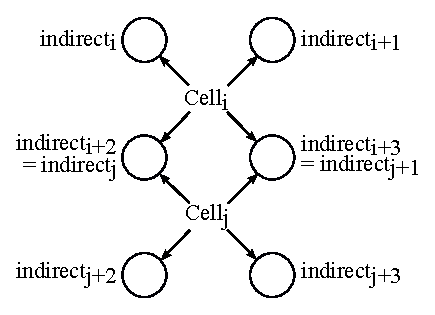
\includegraphics[width=5cm]{fig/svg/mesh2graph.eps}%
    \label{fig:mesh2grapha}%
    }%
  \qquad
  \subfloat[][]{%
    \centering%
    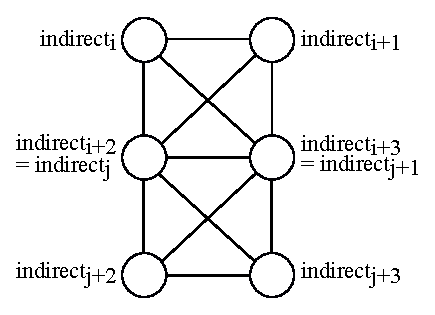
\includegraphics[width=5cm]{fig/svg/mesh2graph_graph.eps}%
    \label{fig:mesh2graphb}%
    }%
  \caption[]{An example of converting a mesh (shown in \subref{fig:mesh2grapha},
  with mapping dimension 4) to a graph (on Figure \subref{fig:mesh2graphb}) for
  the GPS algorithm.}%
  \label{fig:mesh2graph}
\end{figure}

There are several straightforward generalizations to handle multiple sets and
mappings (e.g. vertices, edges, cells and their connections).  The first is to
assume that all the mappings describe a similar topology, so the elements can be
reordered based on only one of the mappings (as described above), then reorder 
the points accessed through the other mappings by, for example, a greedy method.
Another approach could be to reorder every data set separately, and then reorder
the elements based on the new order of the accessed points, combining the
separate data sets (and corresponding mappings) in some way. Since the mappings
in the applications we measured are very similar topologically (in fact, except
for one of the applications we tested, Airfoil, there is only one mapping in 
each application), we used the first method. However, the algorithm fails to 
take into account that on the GPU the threads are grouped into blocks, and data 
reuse can only realistically be exploited within blocks. This results in blocks that are ``pencil-shaped''. The next algorithm 
addresses this limitation.

\subsubsection{Partitioning based reordering}

\noindent To increase data reuse within a block is equivalent to decreasing 
data shared \emph{between} the blocks, more specifically, to decrease the 
number of times the same data is loaded in different blocks (see 
Figure~\ref{fig:unstructured_part}). With the shared memory approach, data needs 
to be loaded only once per block. So the task is to partition the elements into 
blocks of approximately the same size in such a way that when these blocks are 
assigned to CUDA thread blocks, the common data used (loaded into shared 
memory) by different blocks is minimized.

\begin{figure}[Htpb]
  \centering
  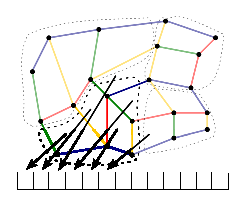
\includegraphics{fig/svg/unstructured_part.eps}
  \caption{Schematic figure of the hierarchical colouring approach with
  partitioning. The thread blocks are circled with dashed lines. The arrows
  represent the individual pieces of data loaded; note that this is less than
  in Figure \ref{fig:unstructured_hier}.}
  \label{fig:unstructured_part}
\end{figure}

Let $G_M$ be a graph constructed from the original mapping, where the points are
the threads, and there is an edge between them if and only if they access the
same data, and let $P_{G_M} = \{B_1, \ldots, B_n\}$ be a partition of this graph
with $n$ blocks. This works even with multiple mappings. If there is a set of 
blocks $B_{d_1}, \ldots, B_{d_k}$ that access the same piece of data, then they 
form a clique in $G_M$ in the sense that between any pair of blocks $B_{d_i}$ 
and $B_{d_j}$ (where $1 \le i,j \le k$), there is an edge of $G_M$ between $u$ 
and $v$ such that $u \in B_{d_i} \wedge v \in B_{d_j}$. Note that the cliques 
have $0.5 \cdot (k^2 - k)$ edges, which is a monotone increasing function in 
$k$, since $k \ge 1$ (there is at least one block writing each data point, 
otherwise it is of no relevance). That means that partitioning using the usual 
objective of minimizing the number of edges between blocks is a good heuristic 
for maximizing data reuse within the blocks.

We chose the k-way recursive partitioning algorithm used by the 
METIS~\cite{metis} library to partition the graph $G_M$. It is a hierarchical
partitioning algorithm, where it first coarsens the graph by collapsing nodes, 
then partitions using the recursive bisection algorithm, and then finally while 
progressively un-coarsening the graph, locally optimizes the cuts. The algorithm 
attempts to maintain equal block sizes in the resulting partition, however, it 
is not always possible because of the underlying algorithm. Since CUDA launches 
thread blocks with equal size, this must be the maximum of the block sizes in 
the created partition. Consequently some threads do not do any work, 
lowering occupancy. One of the tuning parameters for the algorithm is the the 
load imbalance factor, which can be used to specify the tolerance for this 
difference. It is called load imbalance because METIS was originally used 
for distributing computation, ie. load, in a distributed memory system. The 
Load imbalance factor is defined as $l = n\max_j \left\{\mathrm{size}(B_j) 
\right\}$, where $n$ is the number of blocks and $\mathrm{size}(B_j)$ is the 
size of the $j$th block. Due to the local optimization in the un-coarsening 
phase, it is impractical to set this parameter to $1$ (meaning the block sizes 
must be exactly the same). We found that a tolerance of $1.001$ works well in 
practice for our needs.

We design the block size to be a tuning parameter, which specifies the actual
block size of the launched GPU kernels. The number of working threads
cannot exceed the block size. To account for this in partitioning, we calculate 
a new block size ($S'$) and tolerance ($l'$) with margins for the imbalance:
\begin{align}
  S' &= \left\lfloor \frac{S}{l} \right\rfloor \\
  l' &= \frac{S + \epsilon}{S'},
\end{align}
where $S$ is the original block size, $l$ is the original load imbalance
parameter and $\epsilon$ is an empirical tuning parameter to create as large
blocks (within the limit) as possible. This support for a variable number of 
working threads (ie. to determine if the current thread should do any actual 
computation) also incurs a slight overhead of having to load the start and end 
index for each block. We found this overhead to be minimal in practice.

Due to the way loads and stores work on the GPU, what actually affects
performance is not the number of data points accessed, but rather the number of
cache lines (of size 32 bytes on the hardware used) that are accessed. A simple 
heuristic reordering of data points is used to account for this. 

The idea is to group data points together (in a contiguous chunk of memory) that
are read/written by the same set of blocks: this makes them more likely to be
loaded in the same cache line. This is even more important when more blocks
access the same group of data points (set elements on the boundary), since then inefficiencise will worsen
performance for each of these blocks. As a simple heuristic, we group data
points with the same number of blocks that access them together (by sorting),
and within these groups, we sort by the indices of the accessing blocks
lexicographically.

\subsection{Further optimizations}\label{optimisations}

\noindent There are a number of further optimizations we introduced to improve
performance. We can increase the number of loads or stores in flight 
to/from global memory by using CUDA's built-in vector types 
(\lstinline!float2!, \lstinline!float4! and \lstinline!double2!). This way, 
each thread will load multiple consecutive values from memory during a single 
transaction. This is useful to increase the efficiently of loads that are 
already coalesced.

When updating the shared memory with increments, the threads within a block can 
be sorted by their color. Then threads with the same color will be next to each 
other, so warps will have fewer threads of different colors. This results in 
reduced warp divergence on average.

Marking pointers to data on the GPU with \lstinline!\_\_restrict\_\_! and 
\lstinline!const! where applicable enables the compiler to apply further 
reordering optimizations, which it would not have deemed safe to do otherwise. 
\lstinline!\_\_restrict\_\_! instructs the compiler that the pointers do not 
\emph{alias} one another, ie. do not point to the same memory space. The 
\lstinline!const! enables the compiler to place the data in texture cache that 
has lower latency than the global memory.
